\begin{abstract}
We investigate which binary-black-hole population comparisons survive changes in posterior representation, selection-bank representation, and finite numerical integration. The study restores the analysis lineage and original-prior posterior samples for a fixed set of \DataEvents{} public events, comprising \DataRows{} rows. One Phenom-family analysis is selected per event; equal configurations across the catalog are not assumed. A mixed-reference native-tilt diagnostic and a separate negative-effective-spin control are propagated through six fixed models each. In the latter, the inferred binary fraction $g=P(\ceff<0)$ has matched-filter-policy medians from 13.29\% to 28.66\%, with substantially overlapping 90\% credible intervals. At fixed angular shape, changing the spin-magnitude family shifts medians by 12.10--14.34 percentage points. These contrasts remain positive in all \DataReplicates{} paired artificial event/injection thinnings, while a near-zero native-tilt contrast changes sign. We distinguish this finite-bank stability from missing-support uncertainty. An explicit single-event integral-completion family moves some $g$ medians by up to \DataCompletionMax{} points in its limiting case; no completion amplitude is inferred from the samples. We derive conditional posterior envelopes for a bounded unknown log-likelihood correction and quantify when an amplitude-ordering guarantee ceases to hold. Known O3 proposal omissions cannot be certified negligible from a detection-probability bound alone. The results provide a reproducible conditional study and numerical validation, not a measurement of astrophysical formation-channel fractions or a calibration of real-campaign coverage.
\end{abstract}
\noindent\textbf{Keywords:} gravitational waves; binary black holes; population inference; selection effects; importance sampling; reproducibility.

\section{Scientific question and relation to earlier work}
Black-hole formation pathways can predict different masses, spins, redshifts, and correlations. Inferring their branching fractions requires physical population predictions as well as a consistent observational likelihood. A phenomenological alignment component is not a unique formation label. Analyses with multiple physical channels already demonstrate that omitted channels and uncertain physical prescriptions can bias such interpretations \cite{zevin}.

The sensitivity of inferred tilt distributions to model families and priors is established \cite{spinlike}. Common spin reference conventions are also a prior requirement, rather than a new proposal of this study \cite{infinity}. Numerical uncertainty in hierarchical importance sampling has been investigated directly \cite{growing}, including comparisons of injection banks and their thinning \cite{structure}. Requirements on proposal support are explicit in modern injection guidance \cite{injections}. We do not claim these principles, integrated spin summaries, or resampling as new methods.

More recent work recommends integrated angular fractions while showing that even large simulated catalogs can exhibit misleading tilt structure \cite{longroad}. Effective-spin geometry and component-spin modeling assumptions have also been shown to reproduce apparent orientation features \cite{degeneracies}. Event-level spin-prior choices affect numerical convergence and simulated population recovery \cite{spinpriors}. Our normalized sign-shape control does not remove these ambiguities. We do not implement these studies' complete models or claim an independent discovery of prior sensitivity; their problems overlap directly with the interpretation of our results.

Our original question was whether formation-channel interpretations are robust to model assumptions and selection effects. The evidence assembled here supports a necessary, narrower layer of that question: which specified population comparisons survive reconstructing their source arrays and perturbing their numerical banks, and what remains unidentifiable from those banks? This does not replace the eventual physical-channel comparison. The concrete outputs are source connections, reproducible conditional contrasts, an example of reference-dependent derived-field disagreement, and a quantitative separation of retained-bank variability from assumptions about unseen contributions. Independent novelty of these particular instances has not been established.

The present draft supersedes the numerical scope of the project's v0.2 paper, while preserving that version and its frozen products. It is an interim research report: actual omitted-likelihood bounds, a common-reference tilt population analysis, and historical injection-execution details remain open. We do not treat the absence of these ingredients as a successful measurement of channel fractions.

\section{Data and analysis lineage}\label{sec:data}
\subsection{A fixed event set and full-source restoration}
The starting point is the GWPopulation GWTC-3 tutorial \cite{tutorial}. Its arrays provide a useful historical baseline, not a unique representation of the official population analysis. The project retains a fixed set of \DataEvents{} events using its documented search-significance and secondary-mass criteria. Ten initially missing FAR fields were traced to a catalog-merge overwrite and checked against earlier search records; no event is retained merely because its FAR was missing. A count of 69 alone does not establish agreement with another study's membership, classification rule, or waveform choices.

We restore original-prior releases from fixed GWTC-2.1 and GWTC-3 records \cite{pe21,pe3}. The 69 files total \DataBytes{} bytes. Official MD5 values and local SHA-256 hashes were checked. The resulting \DataRows{} rows retain source coordinates, spin azimuths, and available derived fields. Analysis lineage was resolved by row connections and configuration/prior information. Containing labels need not be unique. For one ambiguous analysis, a separately identified cosmological-prior representation provides a three-way connection; another Mixed sample is decomposed into disjoint waveform-origin components. We do not silently use an entire Mixed analysis as a single-waveform posterior.

The selected analyses are in the Phenom family. This does not mean identical waveform versions, likelihood settings, marginalizations, or frequency ranges across all events. Sixty-three files provide the core analytic prior strings inspected here. For six others, released LALInference configurations and fixed historical defaults recover the prior family; all 1,020,789 rows in those six pass the recorded range checks. This is evidence for the density used on released rows, not a reconstruction of every historical command or a bound on likelihood outside the sampling support.

\subsection{Coordinates and priors}
Importance weights use the joint posterior rows, rather than products of marginal distributions or event medians. In the relevant original-prior family, the row-level prior shape in source masses, redshift, magnitudes, and tilt cosines contains
\begin{equation}
 \pi_i^{\rm PE}(\theta)\ \propto\ d_L(z)^2\frac{d d_L}{dz}\,
 \frac{m_1(1+z)^2}{4},\label{eq:prior}
\end{equation}
with event-specific support and constants understood. The mass Jacobian and the isotropic tilt measure must accompany a distance-prior change. Released configuration constraints and the six default-family cases are retained separately. Constants independent of the population parameter cancel within each event's conditional posterior calculation; we do not compare model evidences here.

The prior reconstruction uses the documented flat-$\Lambda$CDM convention $H_0=67.9\,\mathrm{km\,s^{-1}\,Mpc^{-1}}$, $\Omega_m=0.3065$. The fixed target redshift density uses Astropy Planck15. Stored source coordinates are preserved; this is not a cosmological-parameter analysis. A validator that initially failed on valid rows outside the target redshift range was repaired to retain those rows with zero target weight. The failure and repair are recorded; rows are not deleted to make a check pass.

\subsection{Selection inputs and remaining mismatches}
The O3 source is the fixed BBH sensitivity release \cite{o3}. Its accepted bank contains \DataOThreeRows{} rows; accepted is not synonymous with detected. Search statistics define either a union including cWB, or an O3 matched-filter union excluding cWB, with IFAR greater than one year. The latter follows the BBH sensitivity convention discussed in the GWTC-3 population appendix \cite{lvk3}. O1/O2 contributions retain the earlier fixed treatment, including its semianalytic threshold approximation. Our shorthand ``matched-filter policy'' refers to the O3 change; it does not assert a homogeneous, fully reconstructed search law across all runs.

Run times, generated counts, proposal measures, and subset connections were audited. The full O3 representation replaces a smaller combined-file representation, without counting its dependent rows as extra events. Historical execution reference metadata are still not recovered. A later cumulative product also exhibits an early observed-SNR retention floor near 8.5; a compatible truncated-noise model was checked, but that observation does not recover the actual generation configuration. Neither audit certifies full selection consistency.

\section{Conditional population models}\label{sec:models}
\subsection{Fixed mass, redshift, and magnitude assumptions}
The two six-model controls share fixed mass and redshift factors. Primary mass is a 0.9/0.1 mixture of a $m_1^{-2}$ density and a Gaussian of mean $35M_\odot$ and standard deviation $5M_\odot$, both truncated to $[3,100]M_\odot$. At fixed $m_1$, $q=m_2/m_1$ has density proportional to $q$ on $[3M_\odot/m_1,1]$. Redshift has density proportional to $(dV_c/dz)(1+z)$ on $[0,2.3]$. This corresponds to a fixed merger-rate exponent $\kappa=2$ before time dilation; $\kappa$ is distinct from the angular-shape parameter $\lambda$ below. These choices are controls, not newly fitted official mass/redshift distributions.

The spin magnitudes are independently assigned either $\mathrm{Beta}(1.5,8.5)$, called the low-spin family, or $\mathrm{Beta}(2,5)$, called the baseline-amplitude family. The words low and baseline name these two specified distributions; they do not classify observed events. No mass--spin or redshift--spin dependence is fitted. Each model's posterior is conditional on these fixed assumptions; no model averaging is applied.

\subsection{Native-tilt diagnostic}
Let $c_j=\cos\theta_j$ and $A_\sigma(c)$ be a Gaussian centered at one, truncated and normalized on $[-1,1]$. The original angular control is
\begin{equation}
 p(c_1,c_2\mid f,\sigma)=f A_\sigma(c_1)A_\sigma(c_2)+(1-f)/4.
\end{equation}
For the primary-black-hole functional,
\begin{equation}
 r=P(c_1<0)=f A_\sigma^{\rm CDF}(0)+(1-f)/2.\label{eq:r}
\end{equation}
We use $\sigma\in\{0.3,0.6,1.2\}$ and a uniform prior in the common $r$ interval $[\max_\sigma A_\sigma^{\rm CDF}(0),1/2]\simeq[0.34174,0.5]$. It is a genuine support/prior control, not merely a relabeling of the same mixture-parameter posterior.

The native references are 20 Hz for 53 events, 10 Hz for 15, and 16 Hz for one. Consequently this is a mixed-reference numerical diagnostic, not a population measurement of tilts at one common physical reference. It must remain separate from the next functional.

\subsection{Negative-effective-spin control}
Define
\begin{equation}
 x=\ceff=\frac{a_1c_1+qa_2c_2}{1+q},\qquad
 v=\frac{a_1^2+q^2a_2^2}{3(1+q)^2}.
\end{equation}
At fixed $q,a_1,a_2$, use the normalized even angular density
\begin{equation}
 H_\lambda(c_1,c_2)=\frac{1+\lambda x^2}{4(1+\lambda v)},\qquad
 \lambda\in\{0,4,16\}.
\end{equation}
The isotropic mean of $x^2$ is $v$. Simultaneously reversing $c_1,c_2$ leaves $H_\lambda$ unchanged, so each sign domain has probability one half. Thus
\begin{equation}
 p(c_1,c_2\mid g,\lambda)=H_\lambda(c_1,c_2)
 \big[2g\ind_{x<0}+2(1-g)\ind_{x>0}\big]\label{eq:gmodel}
\end{equation}
has $P(x<0)=g$ at every fixed $q,a_1,a_2$. The $x=0$ boundary has measure zero; the implementation supplies a symmetric boundary value. Both magnitude families use a uniform $g\in[0,1]$ prior.

The reference-control interpretation explicitly assumes 2PN conservation of projected effective spin and preservation of the isotropic angular measure during the adopted transport. It is not exact full-GR transport, and the measure-preservation premise is not independently proved here. Released native and infinity-derived $x$ values agree within $5.55\times10^{-16}$ on all rows, with no sign disagreement. These columns are derived from related inputs; their agreement is an implementation check, not independent evidence for a complete physical transport law or the unknown injection reference.

The quantity $g$ describes binaries; $r$ describes the primary black hole. Neither is a mixture weight for a known astrophysical channel. Their different priors and angular model families also prevent interpreting their numerical difference as a direct physical comparison.

\subsection{Likelihood and validation strategy}
With component event means $\mu_{i-},\mu_{i+}$ and efficiencies $\xi_-,\xi_+$, the conditional, rate-free likelihood is
\begin{equation}
 p(g\mid\{d_i\},{\cal M})\propto p(g)
 \frac{\prod_{i=1}^{N}[g\mu_{i-}+(1-g)\mu_{i+}]}
 {[g\xi_-+(1-g)\xi_+]^N},\qquad N=\DataEvents.\label{eq:likelihood}
\end{equation}
The native-tilt calculation uses its corresponding $f(r)$ and components. Event means are estimated by posterior/prior reweighting; efficiencies use the documented proposal densities, run fractions, and generated counts. No event or parameter region is rejected by an ESS threshold. ESS is a contribution-concentration diagnostic and excludes unmeasured PE-chain correlations.

Cartesian-spin source checks, independent prior-distance quadrature, ordinary long-double posterior products, and grid refinements complement the production implementation. Angular normalization and sign probabilities were checked in 120 split-domain quadratures. A separate known-selection/noisy-sign experiment enumerates all 70 counts at $N=69$ and checks prior-averaged coverage. That algorithm test has a maximum coverage discrepancy below $7.6\times10^{-7}$; it is not a real-GW, PE-chain, or injection-campaign coverage experiment.

\section{Full-source and reference results}\label{sec:results}
Restoring all source rows shifts the six native-reference medians by at most \DataMaxSourceShift{} pp relative to the earlier five-full-source baseline, with the other 64 events then represented by tutorial arrays. The low-spin $\sigma=0.3$ minus 1.2 contrast changes from about $+0.18579$ to $\DataNativeLowGap\pp$. The baseline-amplitude contrast is $\DataNativeBaseGap\pp$. Independent full-product quantiles agree within $3.61\times10^{-12}$; this numerical agreement does not repair the mixed references.

\begin{figure}[tbp]
\centering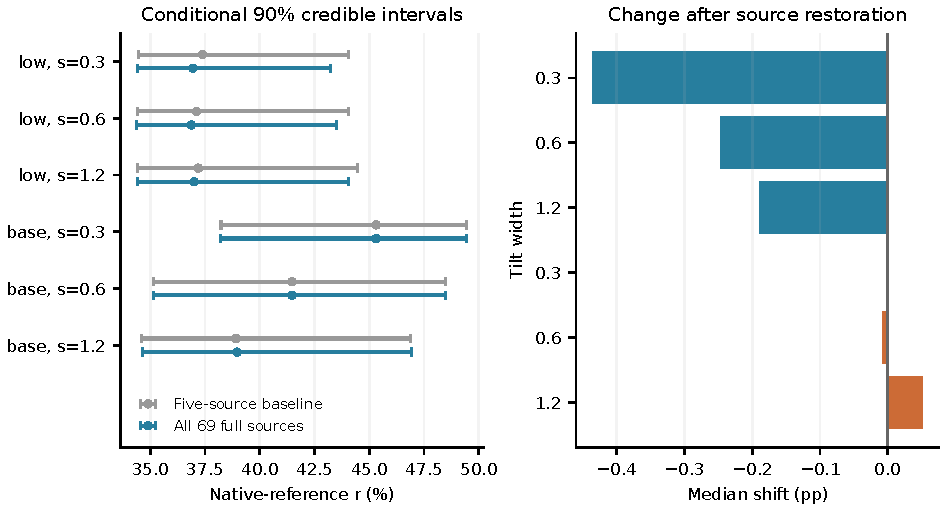
\includegraphics[width=\linewidth]{native-restoration.pdf}
\caption{Native-reference conditional diagnostic before and after all-source restoration. Left: medians and equal-tailed 90\% credible intervals. Right: median displacements on a separate scale. ``Low'' and ``base'' refer to the fixed magnitude distributions. These are not common-reference tilts or channel fractions.}\label{fig:native}
\end{figure}

For the separate $g$ control, Table~\ref{tab:g} gives the matched-filter-policy posterior summaries. At fixed $\lambda$, the amplitude-family median gaps are 12.10, 12.89, and 14.34 pp. The intervals overlap substantially. The gaps do not demonstrate incompatible populations or favor either model by evidence. Omitting selection, as a diagnostic rather than a valid observing model, lowers medians by 5.20--13.86 pp. Adding cWB to the O3 union shifts them by $-0.042$ to $-0.309$ pp. These different axes must not be collapsed into one error estimate.

\begin{table}[tbp]\centering
\caption{Conditional $g$ posteriors. Brackets are equal-tailed 90\% astrophysical credible intervals within each specified model, distinct from the artificial-thinning ranges below.}\label{tab:g}
\begin{tabular}{lrr}
\toprule
Magnitude prior & $\lambda$ & $g$ median [5th, 95th] (\%) \\
\midrule
$\mathrm{Beta}(1.5,8.5)$ & 0 & 13.29 [1.69, 32.27] \\
$\mathrm{Beta}(1.5,8.5)$ & 4 & 13.57 [1.77, 32.57] \\
$\mathrm{Beta}(1.5,8.5)$ & 16 & 14.32 [2.00, 33.33] \\
$\mathrm{Beta}(2,5)$ & 0 & 25.39 [9.26, 43.27] \\
$\mathrm{Beta}(2,5)$ & 4 & 26.47 [10.24, 44.20] \\
$\mathrm{Beta}(2,5)$ & 16 & 28.66 [12.33, 46.06] \\
\bottomrule
\end{tabular}

\end{table}
\begin{figure}[tbp]\centering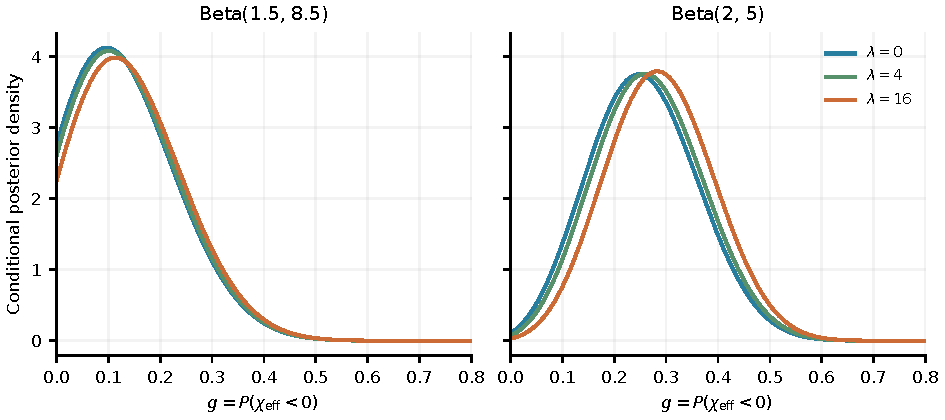
\includegraphics[width=\linewidth]{effective-spin.pdf}
\caption{Conditional $g$ posterior densities for the two magnitude families with the same uniform $g$ prior. Selection, event set, and mass/redshift factors are fixed. The display ends at $g=0.8$; normalization and all calculations use $[0,1]$.}\label{fig:g}
\end{figure}

\subsection{An analysis-label counterexample}
For GW190421\_213856, Phenom and Mixed contain the same 147,856 native posterior points under a complete bijective row connection, but their derived primary infinity-tilt cosine differs by up to 0.12980. The Phenom configuration declares 16 Hz; Mixed lacks the corresponding reference metadata. The recorded PESummary version maps to historical source that supplies 20 Hz when the reference is missing. Independent numerical controls associate the two derived sets with 16 and 20 Hz. Equality of native samples therefore does not ensure equality of their derived reference-dependent columns.

A 20-row diagnosis was followed by 70 distinct held-out/stress rows. One residual of $1.2323\times10^{-6}$ exceeded the original $10^{-6}$ release-agreement gate. Tighter integrations with two solvers agree with each other without removing that discrepancy. Replaying unmodified historical LALSuite 7.0 Python defaults on the same 70 rows reproduces released values within $3.87\times10^{-8}$ and $4.43\times10^{-8}$. This supports a historical-default numerical explanation. It reuses the rows after observing the failure, so it is a follow-up diagnosis, not a new held-out test. The original failed gate remains failed, and the full historical runtime has not been reconstructed.

\begin{figure}[tbp]\centering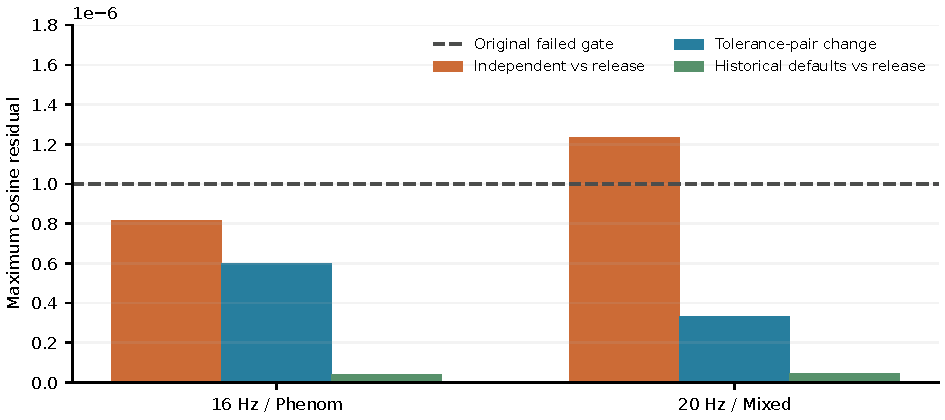
\includegraphics[width=\linewidth]{reference-residual.pdf}
\caption{The original release-agreement failure is retained. Historical-default replay explains the small residual on the same fixed 70-row set; it does not reclassify the independent solver's original test as passing.}\label{fig:reference}
\end{figure}

\FloatBarrier
\section{Paired finite-bank experiments}\label{sec:banks}
\subsection{Design and covariance}
Designs were recorded before these thinning outputs. In each of \DataReplicates{} replicates, each event contributes a simple random sample without replacement of \DataEventDraw{} rows from its complete saved bank. Independently, O3 contributes \DataOThreeDraw{} of its \DataOThreeRows{} accepted rows. The event count stays \DataEvents{}, and O1/O2 contributions remain fixed. Shared indices pair both metrics, all six models, and both policies. Event streams use seed sequence $[20261026,\mathrm{source\ index}]$; O3 uses seed 20261025. Reuse of the earlier O3 random stream is a paired reanalysis, not additional independent replication. The event design does not reproduce historical cosmological-prior rejection sampling.

For a bank of size $M$, a retained sample of size $n$, and vector weights $w_j$, the specified finite-population design has
\begin{equation}
 \operatorname{Cov}(\bar w_n)=\frac{1-n/M}{n}\,
 \frac{1}{M-1}\sum_{j=1}^M(w_j-\bar w_M)(w_j-\bar w_M)^T.\label{eq:cov}
\end{equation}
Event vectors contain 24 entries spanning the two metrics and six component pairs. The O3 vector jointly covers policies as well. Failed-search accepted rows remain zero-weight entries in the sampling frame. Jacobians propagate these joint covariances; direct nonlinear posteriors are calculated separately. This pairing preserves cancellations and interactions that independent error bars would miss.

\subsection{Results and checks}
Table~\ref{tab:finite} and Fig.~\ref{fig:finite} summarize the design. The near-zero native low-spin width contrast is nonpositive in \DataOThreeLowNonpositive\% of O3-only and \DataJointLowNonpositive\% of joint thinnings. These are conditional frequencies of artificial repetitions, not $p$-values. The corresponding event-only, O3-only, and joint standard deviations are 0.17642, 0.49261, and 0.56206 pp. The RMS of the explicit nonlinear interaction
\begin{equation}
 \Delta_{\rm int}=T_{\rm joint}-T_{\rm event}-T_{\rm O3}+T_{\rm full}
\end{equation}
is \DataInteraction{} pp. Linear variances alone do not reproduce every small contrast. The three effective-spin amplitude contrasts remain positive in all 512 joint repetitions; this statement is limited to the specified banks and draw sizes.

\begin{table}[tbp]\centering\small
\caption{Median differences in pp. Native $\Delta r$ is $\sigma=0.3$ minus 1.2; $\Delta g$ is Beta(2,5) minus Beta(1.5,8.5). Brackets are 5th--95th percentiles of the declared artificial thinnings, not credible intervals, confidence intervals, or real-campaign errors.}\label{tab:finite}
\begin{tabular}{lrrrr}
\toprule
Contrast & Full banks & Event only & O3 only & Joint \\
\midrule
$\Delta r$, low spin & -0.060 & [-0.278, 0.289] & [-0.676, 0.932] & [-0.661, 1.075] \\
$\Delta r$, baseline spin & 6.354 & [6.112, 6.637] & [5.548, 7.052] & [5.564, 7.096] \\
$\Delta g$, $\lambda=0$ & 12.098 & [10.412, 13.225] & [9.792, 14.164] & [9.097, 14.333] \\
$\Delta g$, $\lambda=4$ & 12.892 & [11.193, 14.041] & [10.546, 15.001] & [9.871, 15.135] \\
$\Delta g$, $\lambda=16$ & 14.342 & [12.598, 15.522] & [11.874, 16.570] & [11.122, 16.724] \\
\bottomrule
\end{tabular}

\end{table}
\begin{figure}[tbp]\centering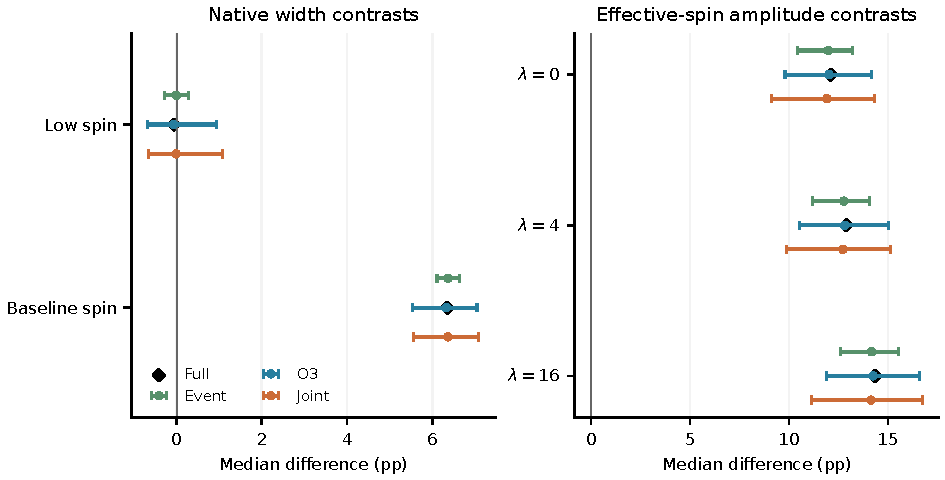
\includegraphics[width=\linewidth]{finite-banks.pdf}
\caption{Artificial-thinning median contrasts. Lines are 5th--95th percentiles; circles are repetition medians; black diamonds use full banks. Fixed O1/O2 and the same 69 observations are used throughout.}\label{fig:finite}
\end{figure}

The independent event validator recomputes source-coordinate means and all 69 finite-bank covariance matrices, checks 512 index-stream fingerprints per source, and directly checks sampled sums at selected repetitions including every contrast extremum. Every event-only and joint posterior product is checked for all 512 repetitions. Maximum quantile discrepancies are $1.53\times10^{-14}$ and $1.40\times10^{-14}$, respectively. This is not a claim that all sampled weight sums were independently recomputed in every repetition.

A second retained numerical failure concerns a weak derivative. A real relative step of $10^{-6}$ gives maximum relative discrepancy $1.04060\times10^{-4}$, above the unchanged $10^{-4}$ gate. The relevant median difference is only about $6\times10^{-12}$, allowing cancellation error. Step $10^{-5}$ passes the same gate with maximum error $4.88\times10^{-6}$; independent fixed-bracket complex differentiation at two steps agrees to $9.51\times10^{-11}$. Production posteriors, draws, and analytic Jacobians were not changed. The original step remains flagged as failed.

\section{Contributions that a bank cannot reveal}\label{sec:support}
\subsection{A conditional posterior-envelope bound}
Let $p(g)$ denote a baseline posterior and let the corrected posterior be proportional to $p(g)h(g)$, with $h>0$. Suppose, without asserting that the data establish it, that
\begin{equation}
 \operatorname*{ess\,sup}_g\log h(g)-\operatorname*{ess\,inf}_g\log h(g)\leq B.\label{eq:B}
\end{equation}
An arbitrary constant in $h$ cancels, so set $1\leq h\leq R=e^B$. For any threshold with baseline CDF value $F$, the smallest corrected mass below it puts weight one below and $R$ above. The largest reverses those weights. Therefore
\begin{equation}
 \frac{F}{F+e^B(1-F)}\leq F_h\leq\frac{e^BF}{1-F+e^BF}.\label{eq:cdf}
\end{equation}
Writing $s(t)=(1+e^{-t})^{-1}$ and $Q$ for the baseline quantile function gives
\begin{equation}
 Q\!\left[s(\operatorname{logit}q-B)\right]\leq Q_h(q)
 \leq Q\!\left[s(\operatorname{logit}q+B)\right].\label{eq:quantile}
\end{equation}
The bounds are sharp over arbitrary positive reweighting functions satisfying Eq.~\eqref{eq:B}. Maximizing the probability shift of a two-domain weighting also yields
\begin{equation}
 \operatorname{TV}(p_h,p)\leq\tanh(B/4).
\end{equation}
Sharpness over this large mathematical class does not establish realizability by one physical waveform likelihood or one detection law shared by all six models.

If the retained integrals were exact and each missing event contribution obeyed a uniform relative bound $\epsilon_i$, while the omitted selection contribution obeyed $\eta_{\rm sel}$ at all $g$, a sufficient budget would be
\begin{equation}
 B=\sum_{i=1}^{69}\log(1+\epsilon_i)+69\log(1+\eta_{\rm sel}).\label{eq:budget}
\end{equation}
Neither resampling nor ESS estimates these bounds. A zero retained integral with a positive completion invalidates a finite uniform relative bound. Bank-internal MC variability is a separate source of error and is not silently included in Eq.~\eqref{eq:budget}.

For an amplitude-model pair, a conservative lower bound on the median difference subtracts the low-amplitude model's upper median envelope from the baseline-amplitude model's lower envelope. Table~\ref{tab:support} lists the $B_*$ at which this certificate reaches zero. If only selection omissions were present, the matched-policy thresholds would correspond to uniform relative bounds of 1.346--1.598\%; the same arithmetic applies if only 69 equal event-omission bounds are present. Both sources cannot each spend the full budget. Loss of a sufficient ordering certificate is not an observed physical reversal.

\begin{table}[tbp]\centering
\caption{Conditional ordering-certificate thresholds. The last column is $100[\exp(B_*/69)-1]$ for the matched policy, under one of the single-source budget interpretations above. No actual missing-contribution bound is estimated.}\label{tab:support}
\begin{tabular}{rrrr}
\toprule
$\lambda$ & $B_*$ matched & $B_*$ with cWB & Equivalent bound (\%) \\
\midrule
0 & 0.92251 & 0.90978 & 1.346 \\
4 & 0.98246 & 0.96835 & 1.434 \\
16 & 1.09371 & 1.07682 & 1.598 \\
\bottomrule
\end{tabular}

\end{table}
\begin{figure}[tbp]\centering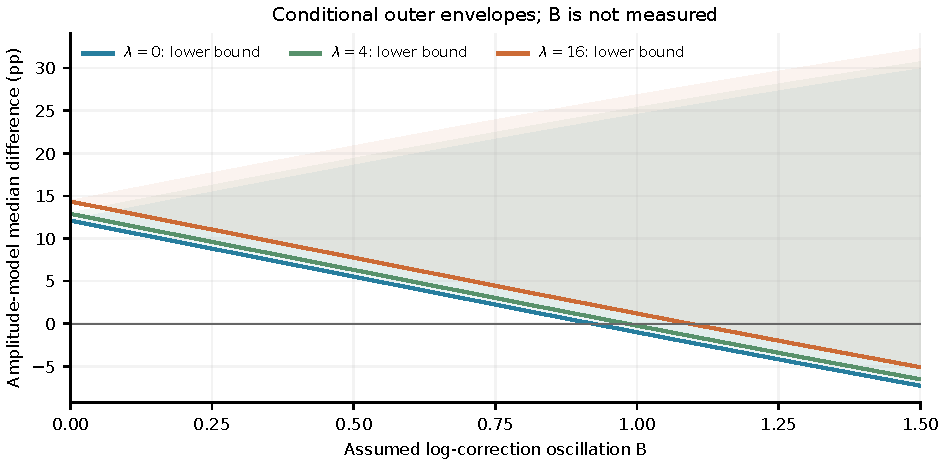
\includegraphics[width=\linewidth]{support-envelope.pdf}
\caption{Outer envelopes for amplitude-model median differences, allowing each model an unknown correction satisfying the same assumed $B$. Shading is a sensitivity envelope, not a credible interval. The underlying baseline posteriors retain their own model assumptions.}\label{fig:support}
\end{figure}

\subsection{A zero-component completion family}
GW191204\_171526 has \DataEventZeroRows{} released rows and zero negative-component weight in all six $g$ models. Its finite-bank sampling covariance cannot generate absent negative contributions. This is not evidence that its physical negative-spin likelihood is zero.

As a declared post-diagnostic stress family, replace only this event's pair $(0,\mu_+)$ by $(\eta\mu_+,\mu_+)$, leaving the other 68 events and selection unchanged. The same $\eta$ is assigned to each model for this illustration. It is an integral ratio, not a missing posterior probability or a fitted parameter. The normalized $\eta\to\infty$ limit uses the negative component alone. Table~\ref{tab:completion} shows the matched-policy response. At $\eta=1$ shifts are 1.23--1.60 pp; the limiting maximum is \DataCompletionMax{} pp. All three amplitude gaps stay positive within this same-$\eta$ family, which is less general than the outer envelopes above. No common physical likelihood is claimed to generate every integral completion.

\begin{table}[tbp]\centering
\caption{One-event completion stress, in pp. The second column spans six model median shifts; the third spans three same-$\lambda$ amplitude gaps. These ranges summarize declared scenarios, not statistical uncertainty.}\label{tab:completion}
\begin{tabular}{rrr}
\toprule
$\eta$ & Median shifts across six models & Three amplitude gaps \\
\midrule
0.0 & [-0.000, 0.000] & [12.098, 14.342] \\
0.01 & [0.014, 0.022] & [12.105, 14.350] \\
1.0 & [1.233, 1.602] & [12.439, 14.649] \\
$\infty$ & [5.201, 8.023] & [9.782, 11.682] \\
\bottomrule
\end{tabular}

\end{table}

\subsection{The known omitted O3 domain and a validation requirement}
The target population assigns \DataTailMass\% of its redshift mass to $1.9<z\leq2.3$, outside the O3 proposal support. The known omitted union also includes either spin magnitude above 0.998; its mass is almost entirely the redshift tail for these two Beta families. Even using only $P_{\rm det}\leq1$, the O3 time-weighted omitted contribution can be bounded above only by about \DataTailBound. This is 137--143 times the represented efficiency near the baseline medians and is far too broad to certify a small selection correction. It bounds the contribution of this stated omitted domain only, not all possible selection biases.

Continuous-cosmology tail integrals and the implemented linearly interpolated density are recorded separately. The bound uses the actual coded measure, including its tiny normalizer offset, so a continuous approximation is not mixed with the represented efficiency. Likewise, small prior mass outside a PE support does not by itself bound an event likelihood integral without additional likelihood information.

A resource calculation makes one possible next experiment concrete. For an assumed 0.5\% uniform selection-completion tolerance, directly draw independent sources from the omitted-domain target conditional on each of six models and two sign components, then evaluate the validated historical O3 union protocol. Under zero detections, exact binomial upper bounds with Bonferroni control over 12 components require \DataTailPlan{} direct draws in total for simultaneous 95\% bounds. This is a planning count, not an executed campaign. Nonzero detections require recomputation. Weighted injection reuse, correlated draws, or a newly chosen protocol do not automatically satisfy this design. Historical reference, noise/time averaging, and search configuration must be established first. Event omissions and represented-bank uncertainty still require their own budgets.

\subsection{Independent support validation}
All nine completion cases, both policies, and six models were checked with ordinary posterior products. Simpson CDFs and direct quantile roots differ from production summaries by at most $2.16\times10^{-7}$ under the fixed $2\times10^{-6}$ gate. An independent solution for the shared point at which the pair of CDFs sums to one reproduces $B_*$ within $1.31\times10^{-6}$. Split-domain quadrature checks the CDF bounds within $2.99\times10^{-7}$. A two-point calculation attains the TV bound. Independent volume quadrature, polynomial antiderivatives for the tabulated measure, and Beta survival integrals check the support masses. These validate algebra and implementation, not the physical value of $B$, $\eta$, or an actual coverage guarantee.

\FloatBarrier
\section{Interpretation and unfinished scientific evidence}
Three distinct conclusions follow. First, source restoration changes a small native-tilt ordering even while absolute median shifts remain below half a percentage point. Second, specified effective-spin amplitude contrasts survive the declared paired finite-bank perturbations. Third, that stability cannot certify robustness to unseen likelihood or detection contributions. The support analysis provides a conditional bound and a stress response rather than filling that evidential gap with a guessed error bar.

The model families are restricted. They fix mass/redshift factors and impose a particular conditional sign/even-shape spin construction. They do not test all allowed mass--spin correlations, compare a library of physical formation channels, or marginalize their theoretical uncertainty. Overlapping within-model credible intervals, surviving median ordering, and inability to guarantee ordering in a wider correction class answer different questions. None alone establishes a channel branching fraction.

The study also leaves common-reference native tilts, actual injection reference/execution details, PE-chain correlations, shared waveform systematics, and actual omitted-likelihood contributions uncalibrated. These are substantive scientific requirements for a stronger physical interpretation, not merely editorial qualifications. This report does not use new catalog releases to relabel a frozen GWTC-3-era dataset as current all-data inference. A future catalog extension needs a fresh source, event-mask, and injection-version audit.

The practical next steps are to constrain missing contributions using likelihood or validated detection experiments, perform explicit physical-channel comparisons with theoretical nuisance choices, and run recovery/coverage tests matched to that end-to-end protocol. Improvements to the visualization cannot substitute for those steps. The workbench should expose the functional, assumptions, reference convention, source provenance, and uncertainty type with every plotted comparison.

\section{Conclusion}
Restoring all original-prior sources and using paired numerical experiments yields a more defensible conditional comparison than treating preprocessed arrays as complete evidence. The small native-tilt ordering is unstable; the selected effective-spin amplitude contrasts are stable under the specified artificial thinning. Their physical robustness beyond retained support remains unestablished. Our quantitative boundaries identify what additional evidence would be needed, while preserving failed checks and avoiding a conversion of phenomenological parameters into formation-channel fractions.

\appendix
\section{Reproduction and evidence map}\label{app:repro}
The code repository is \href{https://github.com/wkryyds4-netizen/blackhole-research-workbench}{Blackhole Research Workbench}. At draft generation, these v0.3 follow-ups are local and not yet pushed; the link is not a claim that the current public HEAD contains them. Large HDF/NPZ files, environments, and third-party source snapshots are retrieved separately. Retrieval URLs, versions, and checksums are retained in the research records. Original code and upstream materials have distinct licensing boundaries.

The scientific entry point is \path{research/population-catalog/README.md}, followed by \path{research/REPRODUCING_POPULATION.md}. Full-source, invariant-control, paired-bank, support, and milestone JSONs identify the precise calculation and independent validator at each layer. The frozen v0.2 inputs are preserved. Do not execute root \path{model.py}: it would replace those frozen products. Importing documented functions is distinct from executing that script. The bytes of \path{run_control.py} participate in its event-integral cache protocol and must be versioned if changed.

For this paper, \path{research/paper/v0.3/build_evidence.py} verifies result/validation hash links and produces the same numerical facts/tables for both languages. It also generates publication-size vector figures. LaTeX sources, figure PDFs, scientific-source hashes, build diagnostics, exported PDF hashes, and rendered-page inspection records accompany the draft. Rebuilding can alter PDF bytes; agreement of hashes alone is not a semantic or scientific validation. The manuscripts are authored in LaTeX and have not been submitted to arXiv; general source preparation follows its documentation \cite{arxivtex}.

The numerical environment for these follow-ups is Python 3.14.5, NumPy 2.4.6, SciPy 1.18.0, Astropy 8.0.1, and Matplotlib 3.11.0. HDF extraction and spin-transport studies use separately documented isolated environments. The later cumulative-release and historical-source diagnostics remain distinct from the exact six-model inputs reported here.

\section*{Attribution and research status}
Chengheng is the research pen name used by the collaborating AI assistant (ChatGPT, OpenAI) in this project. No institutional endorsement is implied. This is an unreviewed computational research draft; the name does not establish eligibility or responsibility requirements for a journal or repository submission. Public GW data and the cited upstream software make the analysis possible. No independent human peer review or new physical formation-channel measurement is claimed.

\begin{thebibliography}{99}
\bibitem{zevin} M. Zevin et al., One Channel to Rule Them All? Constraining the Origins of Binary Black Holes using Multiple Formation Pathways, Astrophys. J. 910, 152 (2021), \href{https://arxiv.org/abs/2011.10057v2}{arXiv:2011.10057v2}.
\bibitem{spinlike} S. Vitale, S. Biscoveanu, and C. Talbot, Spin it as you like: the (lack of a) measurement of the spin tilt distribution with LIGO-Virgo-KAGRA binary black holes, A\&A 668, L2 (2022), \href{https://arxiv.org/abs/2209.06978v3}{arXiv:2209.06978v3}.
\bibitem{infinity} M. Mould and D. Gerosa, Gravitational-wave population inference at past time infinity, Phys. Rev. D 105, 024076 (2022), \href{https://arxiv.org/abs/2110.05507v2}{arXiv:2110.05507v2}.
\bibitem{growing} C. Talbot and J. Golomb, Growing Pains: Understanding the Impact of Likelihood Uncertainty on Hierarchical Bayesian Inference for Gravitational-Wave Astronomy, MNRAS 526, 3495 (2023), \href{https://arxiv.org/html/2304.06138v2}{arXiv:2304.06138v2}.
\bibitem{structure} J. Golomb and C. Talbot, Searching for structure in the binary black hole spin distribution, Phys. Rev. D 108, 103009 (2023), \href{https://arxiv.org/html/2210.12287v2}{arXiv:2210.12287v2}.
\bibitem{injections} R. Essick et al., Compact Binary Coalescence Sensitivity Estimates with Injection Campaigns during the LIGO-Virgo-KAGRA Collaborations' Fourth Observing Run (2025), \href{https://arxiv.org/html/2508.10638v2}{arXiv:2508.10638v2}. O4 conventions in this work are not used to supply missing historical O3 execution metadata.
\bibitem{longroad} S. Vitale and M. Mould, The Long Road to Alignment: Measuring Black Hole Spin Orientation with Expanding Gravitational-Wave Datasets (2025), \href{https://arxiv.org/abs/2505.14875v2}{arXiv:2505.14875v2}.
\bibitem{degeneracies} N. E. Wolfe, A. Hussain, J. Heinzel, and S. Vitale, Binary-black hole spin population results may be driven by prior degeneracies (2026), \href{https://arxiv.org/abs/2609.10753v1}{arXiv:2609.10753v1}.
\bibitem{spinpriors} K. Kobayashi, M. Iwaya, S. Morisaki, K. Hotokezaka, and T. Kinugawa, Impact of Spin Priors on the Population Inference of Merging Binary Black Holes (2026), \href{https://arxiv.org/abs/2602.12509v2}{arXiv:2602.12509v2}.
\bibitem{tutorial} C. Talbot et al., Population inference on GWTC-3, GWPopulation example notebook, \href{https://colmtalbot.github.io/gwpopulation/examples/GWTC3.html}{tutorial}; \href{https://github.com/ColmTalbot/gwpopulation/blob/2daa71e8c56362f2f64e2166a0055478557f239a/examples/GWTC3.ipynb}{commit-pinned source}. Retrieved versions and source hashes are recorded with this project.
\bibitem{pe21} LIGO Scientific Collaboration and Virgo Collaboration, GWTC-2.1 Parameter Estimation Data Release, version v2 (2022), \href{https://zenodo.org/records/6513631}{Zenodo 6513631}. Specific original-prior files and analysis labels are identified in the source manifests.
\bibitem{pe3} LIGO Scientific Collaboration, Virgo Collaboration, and KAGRA Collaboration, GWTC-3 Parameter Estimation Data Release (2021), \href{https://zenodo.org/records/5546663}{Zenodo 5546663}. Use the fixed files/checksums in the source manifests rather than an unspecified latest version.
\bibitem{o3} LIGO Scientific Collaboration, Virgo Collaboration, and KAGRA Collaboration, O3 Search Sensitivity Estimates (2023), \href{https://zenodo.org/records/7890437}{Zenodo 7890437}; fixed file \path{endo3_bbhpop-LIGO-T2100113-v12.hdf5}.
\bibitem{lvk3} LIGO Scientific Collaboration, Virgo Collaboration, and KAGRA Collaboration, The population of merging compact binaries inferred using gravitational waves through GWTC-3, Phys. Rev. X 13, 011048 (2023), \href{https://arxiv.org/abs/2111.03634v3}{arXiv:2111.03634v3}, Appendix A.
\bibitem{arxivtex} arXiv, Submit TeX/LaTeX, \url{https://info.arxiv.org/help/submit_tex.html}, consulted 25 October 2026. This draft has not been submitted to arXiv.
\end{thebibliography}

